% Metódy inžinierskej práce

\documentclass[10pt,twoside,slovak,a4paper]{article}

\usepackage[slovak]{babel}
%\usepackage[T1]{fontenc}
\usepackage[IL2]{fontenc} % lepšia sadzba písmena Ľ než v T1
\usepackage[utf8]{inputenc}
\usepackage{graphicx}
\usepackage{url} % príkaz \url na formátovanie URL
\usepackage{hyperref} % odkazy v texte budú aktívne (pri niektorých triedach dokumentov spôsobuje posun textu)

\usepackage{cite}
%\usepackage{times}

\pagestyle{headings}

\title{Vývoj crossplatformových (OS) aplikácii\thanks{Semestrálny projekt v predmete Metódy inžinierskej práce, ak. rok 2015/16, vedenie: Vladimír Mlynárovič}}

\author{Ignác Borový\\[2pt]
	{\small Slovenská technická univerzita v Bratislave}\\
	{\small Fakulta informatiky a informačných technológií}\\
	{\small \texttt{...@stuba.sk}}
	}

\date{\small 19. october 2021}



\begin{document}

\maketitle


\section{Úvod} \label{Uvod}
\quad
Keďže tu máme rôzne typy zariadený mobily, tablety, počítače a atd.. Tak na tieto zariadenia existuje veľa rôznych operačných systémov ako je Windows, Linux, Android a ďalšie. Tu nám vzniká problém ako vyvinúť software tak aby fungoval na všetky tieto operačné systémy, keďže každý systém na inakšiu architektúru a nástroje. 

Riešením je crossplatformový vývoj. Zamerám sa hlavne na to ako sa technologie vysporiadavajú s týmto problémov prenositeľnosti. Čiže sa budem zaoberať ako aplikácia dokáže nezávisle fungovať od platformy, akú architektúru takéto aplikácie používajú a ako taký kód vo finále vyzerá.
\cite{Crossplatform}

\section{Prenositeľnosť}
\subsection{Výhody a nevýhody}

\quad
Softwerova prenositeľnosť ale portovanie softwaru ma rôzný význam pre rôzných ľudí. V našom prípade sa jedná o prenositeľnosť softwaru medzi rôznymi platformami v našom prípade OS. Najväčšia výhoda platformovej prenositeľnosti je že dokážeme väčšiu skupinu uživateľov ktorý používaju rôzne operačné sýstemy. 
Ďalšími výhodami sú:
\begin{itemize}
    \item menšia cena za vývoj aplikácie
    \item ľahší vývoj a ľahšie údržba aplikácie.
\end{itemize}
Nevýhody:
\begin{itemize}
    \item pomalšia rýchlosť aplikácie
    \item väčšia veľkosť aplikácie
\end{itemize}

\subsection{Platformová nezávislosť programovacím jazykom} \label{PlatformovaNezavislost}

\quad
Našim cieľom je dosiahnuť aby softwer mohol fungovať nezávisle od hardwaru stroja alebo operačného systému.
\quad
Vhodným jazykom na vývoj tohto softwéru je interpretovaný programovací jazyk JAVA. Interpretovaný jazyk je jazyk ktorý nekompiluje kód do zdrojového kódu ale do takzvaného \textbf{medzikódu} (ByteCode). Výhodou tohoto je, že tento mezikód je spustani na virtuálním stroji Javy (JVM - Java Virtual Machine). Program teda stačí napísat iba raz a môžme ho spustiť všade kde je nainštalovaní JVM.


Toto so sebou aj prináša že, aplikácie sú značne pomalejšie, oproti natívnym aplikáciam. Aby sa vyhlo tejto pomalosti, vyvinula firma Sun takzvaný \textbf{Just In Time Compiler} (JIT). Ten zrychluje aplikácie tak, že mezikód prekládá do strojového kódu procesoru. Správa paměti je zabezpečena pomocí automatického garbage collectoru. Ten vyhladá nepoužívané časti pamäti a uvolňuje ju.
\cite{Java}

\begin{figure}[!ht]
    \centering
    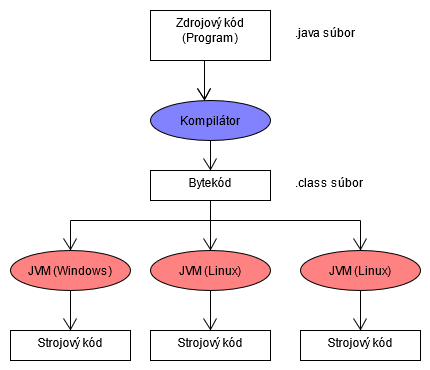
\includegraphics[scale=0.6]{javaByteCode.png}
    \caption{Kompilácia java kódu do ByteKódu a jeho spuštanie na jednotlivých platformách}
\end{figure}


%\acknowledgement{Ak niekomu chcete poďakovať\ldots}


\bibliography{bibliografia}{}
\bibliographystyle{plain}
\end{document}
